\chapter{Implementación}

Ya teniendo todo planificado y sabiendo que metodologías vamos a seguir, 
empezaremos con la implementación de la solución. Lo primero, por supuesto, es 
haber creado nuestro \href{https://github.com/jero-dev/proyecto-tfg}
{repositorio en GitHub} donde subir todos los progresos que hagamos no solamente en 
el propio desarrollo de la solución, sino también en la redacción de la memoria del 
trabajo.

En cuanto a los otros elementos que hemos mencionado como las 
\href{https://github.com/jero-dev/proyecto-tfg/issues}{issues}, los 
\href{https://github.com/jero-dev/proyecto-tfg/milestones}{milestones} y 
\href{https://github.com/users/jero-dev/projects/1}{nuestro tablero Kanban}, se 
pueden encontrar en los enlaces que se encuentran en este párrafo.

Con todo esto ya realizado, es momento de empezar a identificar las historias de 
usuario que podemos encontrar gracias a la definición de personas que llegamos a 
realizar en el capítulo de introducción.

\section{Historias de usuario}

Habiendo identificado los distintos usuarios que hemos encontrado, podemos 
desarrollar las historias de usuario relacionadas o casos de uso que se pueden 
desarrollar para este proyecto. Para ello, hemos definido las siguientes historias:

\subsection{[HU01] Buscar videojuegos por nombre}

Como persona menor de 20 años/coleccionista, quiero poder buscar un videojuego por 
su nombre para obtener las distintas tiendas que lo venden y su precio, además de 
su enlace de compra para cada una.

\textbf{Condiciones de satisfacción}:

\begin{itemize}
    \item La solución debe de poder buscar un videojuego por su nombre.
    \item La solución debe de poder obtener las distintas tiendas que venden el 
    videojuego.
    \item La solución debe de poder obtener el precio de cada tienda.
    \item La solución debe de poder obtener el enlace de compra del videojuego para 
    cada tienda.
\end{itemize}

\subsection{[HU02] Obtener avisos automáticos acerca de un videojuego}

Como coleccionista, tendría en cuenta la opción de obtener avisos automáticos de la 
disponibilidad de un videojuego en concreto en el que tengo interés.

\textbf{Condiciones de satisfacción}:

\begin{itemize}
    \item La solución debe de ofrecer avisos automáticos de la disponibilidad de un 
    videojuego.
    \item En el aviso debe de aparecer el precio de cada tienda.
    \item En el aviso debe de aparecer el enlace de compra del videojuego para 
    cada tienda.
\end{itemize}

En nuestro caso nos centraremos principalmente en la primera historia de usuario, 
completando la segunda en caso de que tengamos tiempo suficiente para ello.

\section{Diseño de la aplicación}

Teniendo ya las historias de usuario, vamos a empezar a diseñar la solución. Para 
ello, seguiremos el diseño dirigido por dominios (en inglés, Domain Driven Design o 
DDD) \cite{ddd} para identificar de manera correcta el dominio del problema y poder 
así concentrarnos totalmente en él.

\begin{itemize}
    \item \textbf{Dominio del problema:} Tenemos como dominio del problema la 
    gestión de ofertas y promociones de productos (aunque nos centremos en 
    videojuegos). En cuanto a los conceptos (entidades) que hemos identificado, 
    tenemos solamente uno: el de \textbf{videojuego}. Aparte, tenemos también un 
    ``value object'' que sería el de \textbf{oferta} y un agregado de ambos que es 
    el de \textbf{producto}.
    \begin{itemize}
        \item \textbf{Videojuego}: Las propiedades de esta entidad serían un 
        \textbf{identificador único}, el \textbf{nombre} del producto y la 
        \textbf{plataforma} en la que se juega.
        \item \textbf{Oferta}: Las propiedades de este ``value object'' serían el 
        \textbf{precio} y el \textbf{enlace} a la tienda donde se encuentra la 
        oferta.
        \item \textbf{Producto}: Las propiedades de este agregado serían un 
        \textbf{videojuego} y una \textbf{lista de ofertas} que se han encontrado 
        para este.
    \end{itemize}
    \item \textbf{Contexto delimitado:} Para centrarnos en el problema, tenemos que 
    delimitar el contexto del mismo. Aquí tenemos claro que el contexto es la 
    gestión de ofertas.
    \item \textbf{Servicios de dominio:} Los servicios de dominio encapsulan la 
    lógica de negocio que no pertenece a ninguna entidad o valor. Aquí podemos 
    encontrar dos claros servicios de dominio: el procesamiento de los mensajes y 
    la gestión de las ofertas.
\end{itemize}

Teniendo el análisis realizado, podemos plasmarlo directamente a la estructura de 
nuestra aplicación. Primero, crearemos un directorio llamado \verb|entity| donde 
guardaremos la entidad \verb|VideoGame| con las propiedades mencionadas. Después, 
añadimos otro directorio llamado \verb|value_object| donde guardaremos el ``value 
object'' de \verb|Offer| también con sus propiedades apropiadas.

Este tipo de datos son básicos, sin ningún tipo de método fuera de un constructor y 
dos métodos de acceso para las propiedades de \verb|Offer|. Por ello, no vamos a 
tener pruebas unitarias para ellos.

Siguiendo con los conceptos que hemos identificado, queda el agregado de 
\verb|Product|. Este va a estar contenido en otro directorio llamado 
\verb|aggregate| en el que encontraremos tanto el tipo \verb|Product| como también 
las pruebas unitarias para el mismo en dos ficheros: \verb|product.go| y 
\verb|product_test.go|.

Necesitaremos guardar estos datos de alguna manera, así que añadiremos otro 
directorio llamado \verb|domain| que contendrá otro llamado \verb|product|. Aquí 
tendremos una interfaz que será la responsable de crear el contrato de cómo se debe 
de comportar un repositorio (por ello llamaremos al fichero \verb|repository.go|) 
para que no tengamos que depender de una tecnología en concreto. 

Para tener nuestro producto mínimamente viable, generaremos primero un repositorio 
en memoria que, si finalmente tenemos tiempo, podremos cambiar por uno que se 
conecte a una base de datos de nuestra preferencia. Con ello, tendremos otro  
directorio llamado \verb|memory| con dos ficheros: \verb|memory.go| y su respectivo 
fichero de pruebas unitarias \verb|memory_test.go|.

Finalmente, llegamos a los servicios de dominio. Añadimos un directorio llamado 
\verb|service| que contendrá los distintos casos de uso o servicios. Uno se llamará 
\verb|offer_manager.go| y otro será \verb|message_processor.go|. Al ser una lógica 
más compleja, dejaremos la implementación de estos para la siguiente sección. 
También añadiremos el fichero principal de esta aplicación que llamaremos 
\verb|api.go|, ya que es lo que al final será esta aplicación: una API.

\section{Procesamiento de mensajes}

Como hemos mencionado, el servicio de procesamiento de mensajes tiene una lógica 
más compleja, por el hecho de que tiene que encontrar el videojuego que se 
encuentra en el mensaje junto con la oferta mencionada en el mismo. Primero de 
todo, necesitamos ver cómo es el tipo de mensajes que se encuentran en los canales 
de ofertas. En la figura \ref{fig:ejemplo de oferta} se puede ver uno de los 
mensajes de los principales canales de ofertas:

\begin{figure}[h]
    \centering
    
\includegraphics[scale=0.5]{figuras/ejemplo-ofertasjuegos.png}
    \caption{Ejemplo de una notificación de oferta.}
    \label{fig:ejemplo de oferta}
\end{figure}

La mayoría de mensajes que se encuentran en los canales de ofertas tienen el mismo 
formato, así que podemos aprovechar esta característica para llegar a procesarlos 
con una expresión regular.

Dentro del fichero \verb|message_processor.go| crearemos una interfaz llamada 
\verb|MessageProcessor| que declarará solamente un método público que hará la 
interpretación de datos: \verb|ParseMessage|. Este método recibirá el mensaje y 
devolverá el nombre del videojuego, la plataforma, el precio y el enlace de compra.

Para ello, implementaremos el método dentro de una estructura que siga el contrato 
de la interfaz. Esta estructura se llamará \verb|MessageProcessorService| que 
implementará la interfaz mencionada. En el método utilizaremos tres expresiones 
regulares para encontrar los campos:

\begin{itemize}
    \item \verb|gameRegex|: Esta expresión regular busca un patrón que comienza 
    con un emoji de flecha hacia abajo, seguido de un conjunto de caracteres que no 
    contienen '\#', luego '\#', y finalmente, una cadena de caracteres de palabra 
    (letras, dígitos o guiones bajos) después de '\#'.
    \item \verb|priceRegex|: Esta expresión regular busca la presencia de 
    ``BAJONAZO'' o ``FLASH'' seguido de un precio expresado en euros.
    \item \verb|linkRegex|: Esta expresión regular busca cualquier URL que comience 
    con 'http://' o 'https://', seguido de cualquier secuencia de caracteres no 
    espaciados.
\end{itemize}

Esta implementación se ha hecho y comprobado gracias a haber realizado las pruebas 
unitarias desde el principio, utilizando un grupo de nueve casos de prueba para que 
el método funcione como se espera. Estos nueve casos son mensajes reales que se han 
encontrado en el canal de \href{https://ofertasjuegos.es/}{Ofertas Juegos}, uno de 
los grupos de canales más populares de ofertas de videojuegos en Telegram.

En cuanto a por qué hemos creado una interfaz para este servicio, es por el hecho 
de que en el futuro nos ayudará para crear pruebas unitarias de manera más 
sencilla, pero eso lo veremos en una de las próximas secciones.

\section{Gestión de ofertas}

Ya con la lógica de procesamiento de mensajes implementada, pasamos al otro 
servicio de dominio, que es el de gestión de ofertas. Este servicio se encargará de 
tanto añadir una oferta como de obtener las ofertas de un título en concreto en 
todas las plataformas.

Este servicio tendrá dos métodos: \verb|StoreOffer| y \verb|GetGameOffers|. El 
primero añadirá una oferta a un producto, mientras que el segundo devolverá las 
ofertas de un videojuego en todas las plataformas en la que esté disponible.

A la hora de implementar la lógica de \verb|StoreOffer|, debemos de comprobar si el 
producto existe en el repositorio. Si este no existe, se genera y añadiremos la 
oferta que se menciona. Si existe, obtenemos la oferta y la añadimos al producto. 
En el caso de añadir la oferta, se verificaba de por sí si el enlace al producto en 
la tienda en el método \verb|AddOffer| del agregado de producto, y solamente se 
actualiza el precio.

Es por esto que vamos a necesitar un nuevo método en el repositorio para devolver 
el producto que coincide con el nombre y la plataforma que se le pasa como 
parámetros. Para ello, añadimos el método \verb|FindByNameAndPlatform| a la clase 
\verb|ProductRepository|. Por supuesto, se pueden encontrar las pruebas unitarias 
relacionadas en el fichero \verb|memory_test.go|.

Ya con el nuevo método, vamos a implementar el servicio de almacenamiento de 
ofertas. Tendremos un nuevo método llamado \verb|StoreOffer| que recibirá el nombre 
del videojuego, la plataforma de este, el precio de la oferta y el enlace donde 
encontrarla.

Teniendo el almacenamiento de las ofertas, vamos a implementar la devolución de las 
ofertas de un videojuego en todas sus plataformas. Pero, todavía no tenemos otro 
método necesario en la capa de repositorio: necesitamos encontrar las ofertas por 
solamente el nombre del videojuego. Este método se llamará \verb|FindByName|.

Con esto ya hecho, podemos implementar el método \verb|GetGameOffers| que recibirá 
el nombre del videojuego y devolverá las ofertas de este en todas sus plataformas.

Ya teniendo la lógica de negocio implementada, podemos pasar a la parte de la 
infraestructura de la solución.

\section{Infraestructura}

Como hemos mencionado anteriormente, queremos que la solución sea una API. Sin 
embargo, esta no va a encargarse de todo (recibir los mensajes desde Telegram y 
demás servicios de mensajería, además de la lógica de negocio), sino que va a tener 
única y exclusivamente dos entradas: una para recibir una cadena de texto que sería 
el mensaje de una oferta y otra para devolver las ofertas de un videojuego dado.

Y entonces, ¿cómo vamos a gestionar la recepción de los distintos servicios de 
mensajería? Lo que haremos será crear otra API por cada bot para servicio de 
mensajería que queramos utilizar. En la figura \ref{fig:infraestructura} se puede 
ver un diagrama de la infraestructura.

El por qué de esta infraestructura es por el hecho de que, si en el futuro se 
quieren añadir más servicios de mensajería, solamente se tendría que añadir un
nuevo bot que se encargue de recibir los mensajes y enviarlos a la API principal.
Además, nos permite tener una mayor fiabilidad en el caso de que alguno de los bots 
deje de funcionar por algún problema, ya sea por la plataforma de despliegue o por 
algún problema con el servicio de mensajería, haciendo que la API no dependa de 
ello.

\begin{figure}[h]
    \centering
    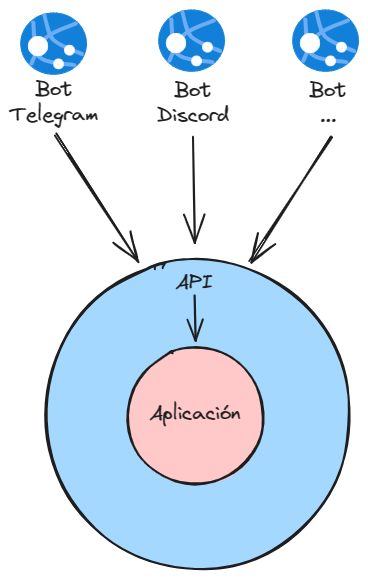
\includegraphics[scale=0.5]{figuras/infraestructura-solucion.png}
    \caption{Infraestructura de la solución.}
    \label{fig:infraestructura}
\end{figure}

Las dos entradas junto con la función principal con la configuración de la API se 
encuentran en el fichero \verb|api.go|. Además, se ha añadido otro fichero llamado 
\verb|api_test.go| para las pruebas de integración de la API.

Para el despliegue, hemos revisado varios servicios de hosting de aplicaciones. Se 
han valorado los más comunes como Heroku, AWS, Azure y Google Cloud Platform, pero 
finalmente nos hemos decidido por usar \href{https://www.fl0.com}{FL0} para 
este caso, ya que tiene integrado un servicio de despliegue continuo directamente 
con GitHub y es de uso gratuito para proyectos de pequeña escala.

\section{Obtención de mensajes de canales de Telegram}

Teniendo nuestra aplicación principal terminada, necesitamos ahora obtener los 
mensajes directamente de los canales de Telegram. Para esto, vamos a crear un bot 
de Telegram que llamaremos \verb|VidyaSale Collector| que se encargará de recibir 
y procesar los mensajes de los canales de ofertas en donde esté. Este bot 
utilizará la librería 
\href{https://github.com/go-telegram-bot-api/telegram-bot-api}{Telegram Bot API} 
para las conexiones con la API de Telegram. Con ella, el desarrollo del bot es 
mucho más ligero que si lo tuviéramos que hacer por nuestra cuenta, ofreciéndonos 
configuraciones de base para el bot y realizar las acciones que necesitemos.

Para el manejo de actualizaciones (mensajes nuevos, ediciones de mensajes, etc.), 
se pueden emplear dos métodos: \verb|GetUpdates| y \verb|Webhook|. El primero 
llama constantemente a la API de Telegram preguntando si hay alguna actualización, 
haciendo que el número de llamadas sea muy alto y haciendo que posiblemente el 
costo en el despliegue a producción aumente.

Es por eso que nos hemos decantado por usar el método \verb|Webhook|, que contacta 
con la API de Telegram informando de que, si el bot recibe alguna actualización, se 
le envíe a una URL en concreto. En la figura \ref{fig:metodos_actualizacion} se 
puede ver una simplificación de cómo funcionan ambos métodos.

\begin{figure}[h]
    \centering
    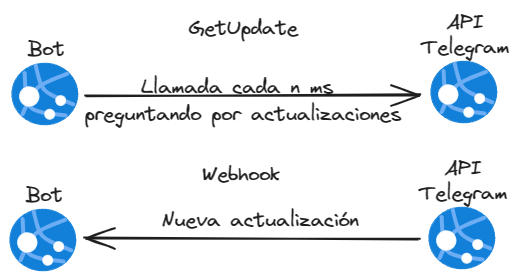
\includegraphics[scale=0.55]{figuras/metodos-actualizacion.png}
    \caption{Métodos de recepción de actualizaciones de Telegram.}
    \label{fig:metodos_actualizacion}
\end{figure}

Al haber elegido el segundo método, necesitamos que el bot esté desplegado en un 
servidor que tenga una URL pública, ya que si no, no se podría conectar con este. 
Para ello, utilizaremos la misma plataforma para el despliegue que hemos utilizado 
para la API principal.

Para terminar, lo que hará el bot será comprobar que tipo de mensaje es el que se 
ha recibido (si viene de un canal o de un grupo, si es un mensaje nuevo o una 
edición de un mensaje, etc.) y, si es un mensaje nuevo de un canal, se procesará 
para enviarlo a la API principal para que lo procese y almacene la oferta.

\section{Interacción del usuario con la solución}

Con los servicios ya recolectando los mensajes de los canales y almacenando la 
información obtenida después de procesarlos, necesitamos que el usuario pueda 
usarlo de una manera sencilla.

Hay varias opciones para esto, pero por ahora hemos decidido crear otro bot con el 
que el usuario se pueda comunicar y que este le devuelva la información relacionada 
con lo que el usuario le pida. Esto es por tener cuanto antes una opción que pueda 
ser utilizado por los usuarios finales y también por ser un desarrollo muy parecido 
al del bot que se encarga de recolectar los mensajes de los canales.

\begin{figure}[h]
    \centering
    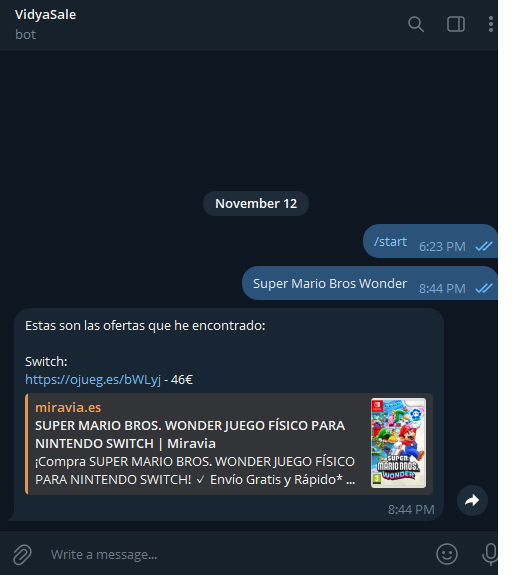
\includegraphics[scale=0.6]{figuras/respuesta-bot.png}
    \caption{Respuesta al preguntar por un título.}
    \label{fig:respuesta_bot}
\end{figure}

Lo que debe de hacer el usuario es enviar un mensaje al bot con el nombre del 
videojuego en el que esté interesado y el bot le devolverá un mensaje con las 
ofertas de este en las plataformas que encuentre. En la figura 
\ref{fig:respuesta_bot} se puede ver un ejemplo de la respuesta del bot cuando se 
le pregunta por un título.

Con esto, ya tenemos la solución que puede ser usada perfectamente por los usuarios 
ya identificados al inicio de este documento.